\documentclass[11pt]{article}

\usepackage[margin=1in]{geometry}
\usepackage[T1]{fontenc}
\usepackage[utf8]{inputenc}
\usepackage{lmodern}
\usepackage{microtype}
\usepackage{amsmath,amssymb,amsthm,mathtools,bm}
\usepackage{booktabs,array,longtable}
\usepackage{xcolor}
\usepackage{hyperref}
\usepackage[most]{tcolorbox}
\usepackage{tikz}
\usepackage{pgfplots}
\usepackage{tikz-3dplot}
\usepackage{enumitem}
\usepackage{caption}
\usepackage{float}
\usepackage{fancyhdr}
\usepackage{titlesec}

\pgfplotsset{compat=1.18}
\usetikzlibrary{arrows.meta,calc,positioning,matrix,fit,backgrounds,decorations.pathreplacing,shapes.geometric}

\hypersetup{
  colorlinks=true,
  linkcolor=blue!60!black,
  urlcolor=blue!60!black,
  citecolor=blue!60!black,
  pdftitle={Chapter 10. Chain Rule, Jacobians, and Automatic Differentiation}
}

\setlength{\headheight}{14pt}
\setlength{\parindent}{0pt}
\setlength{\parskip}{0.65em}
\setlist[itemize]{topsep=2pt,itemsep=2pt}
\setlist[enumerate]{topsep=2pt,itemsep=2pt}
\titleformat{\section}{\large\bfseries}{\thesection}{0.6em}{}
\titleformat{\subsection}{\normalsize\bfseries}{\thesubsection}{0.6em}{}

\pagestyle{fancy}
\fancyhf{}
\lhead{Chapter 10. Chain Rule, Jacobians, and Automatic Differentiation}
\rhead{\thepage}
\renewcommand{\headrulewidth}{0.4pt}

\newtcolorbox{chapteroverviewbox}{
  enhanced,breakable,
  colback=blue!4,
  colframe=blue!55!black,
  boxrule=0.7pt,
  arc=2mm,
  left=2mm,right=2mm,top=1mm,bottom=1mm
}

\newtcolorbox{goalbox}{
  enhanced,breakable,
  colback=green!4,
  colframe=green!45!black,
  title=Learning goals,
  fonttitle=\bfseries,
  boxrule=0.7pt,
  arc=2mm
}

\newtcolorbox{importantbox}[1][]{
  enhanced,breakable,
  colback=red!3,
  colframe=red!60!black,
  title=#1,
  fonttitle=\bfseries,
  boxrule=0.7pt,
  arc=2mm
}

\newtcolorbox{notebox}[1][]{
  enhanced,breakable,
  colback=blue!3,
  colframe=blue!50!black,
  title=#1,
  fonttitle=\bfseries,
  boxrule=0.7pt,
  arc=2mm
}

\newtcolorbox{warningbox}[1][]{
  enhanced,breakable,
  colback=yellow!8,
  colframe=orange!75!black,
  title=#1,
  fonttitle=\bfseries,
  boxrule=0.7pt,
  arc=2mm
}

\newtcolorbox{formulabox}[1][]{
  enhanced,breakable,
  colback=gray!5,
  colframe=gray!70!black,
  title=#1,
  fonttitle=\bfseries,
  boxrule=0.6pt,
  arc=1.5mm
}

\newcounter{workedexamplecounter}
\renewcommand{\theworkedexamplecounter}{10.\arabic{workedexamplecounter}}
\newtcolorbox{workedexample}[1][]{
  enhanced,breakable,
  colback=white,
  colframe=blue!65!black,
  colbacktitle=blue!65!black,
  fonttitle=\bfseries,
  title={Worked example~\theworkedexamplecounter: #1},
  before upper={\refstepcounter{workedexamplecounter}},
  boxrule=0.7pt,
  arc=1.5mm,
  left=2mm,right=2mm,top=1mm,bottom=1mm
}

\newcommand{\R}{\mathbb R}
\newcommand{\grad}{\nabla}
\newcommand{\dd}{\,d}
\newcommand{\Jac}{J}
\newcommand{\bmat}[1]{\begin{bmatrix}#1\end{bmatrix}}

\begin{document}

\begin{center}
  {\LARGE\bfseries Chapter 10. Chain Rule, Jacobians, and Automatic Differentiation\par}
  \vspace{0.3em}
  {\large Compositions, sensitivity, computational graphs, and backpropagation\par}
\end{center}

\begin{chapteroverviewbox}
The chain rule is the rule for differentiating a function built from other functions. In single-variable calculus, if $y=f(u)$ and $u=g(t)$, then
\[
\frac{dy}{dt}=\frac{dy}{du}\frac{du}{dt}.
\]
In multivariable calculus, the same idea becomes more powerful because each intermediate quantity may depend on several variables, and each output may have several components. The derivative is no longer just one number. It may be a gradient vector, a Jacobian matrix, or a linear transformation.

This chapter is one of the main bridges from classical multivariable calculus to modern computation. The chain rule explains how input changes propagate through a model, why Jacobian matrices describe local sensitivity, how coordinate transformations are differentiated, and why backpropagation in neural networks is repeated use of the chain rule.
\end{chapteroverviewbox}

\begin{importantbox}[Core principle]
The multivariable chain rule says that derivatives propagate through compositions by multiplying the correct local linear maps.
\end{importantbox}

\begin{notebox}[Teaching-material connection]
This chapter develops partial derivatives, gradients, tangent-plane approximation, directional derivatives, and implicit differentiation into a systematic treatment of chain rules and Jacobians. The same notation later supports change of variables, optimization, statistics, machine learning, and vector calculus.
\end{notebox}

\begin{goalbox}
After studying this chapter, you should be able to:
\begin{enumerate}
  \item recognize compositions of one-variable, two-variable, and vector-valued functions;
  \item apply the chain rule when $z=f(x,y)$ and $x=x(t)$, $y=y(t)$;
  \item apply the chain rule when $z=f(x,y)$ and $x=x(s,t)$, $y=y(s,t)$;
  \item compute Jacobian matrices for maps $F:\R^n\to\R^m$;
  \item write the multivariable chain rule in matrix form;
  \item interpret the Jacobian as the local linear map of a nonlinear function;
  \item compute and verify Jacobians numerically using finite differences;
  \item understand computational graphs as organized compositions;
  \item explain reverse-mode automatic differentiation and backpropagation at a conceptual level.
\end{enumerate}
\end{goalbox}

\section{Why composition matters}

A function of several variables often appears indirectly. For example, suppose
\[
z=f(x,y)=x^2y+\sin y,
\]
but $x$ and $y$ themselves depend on time:
\[
x=t^2,\qquad y=e^t.
\]
Then $z$ is ultimately a function of $t$:
\[
z(t)=f(x(t),y(t))=t^4e^t+\sin(e^t).
\]
We could substitute first and then differentiate. But in applications, substitution may be inconvenient or impossible. The chain rule computes the derivative by following the dependencies.

\begin{figure}[H]
\centering
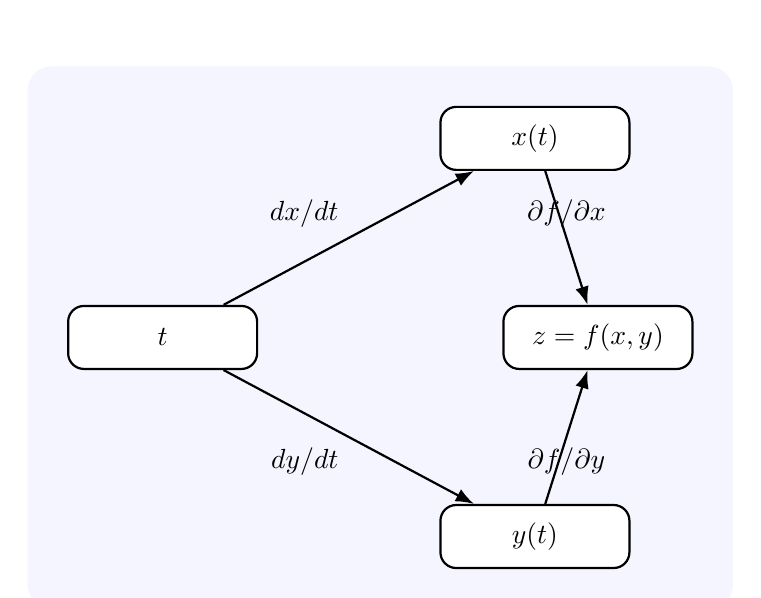
\begin{tikzpicture}[
  node distance=1.7cm and 2.3cm,
  box/.style={draw,rounded corners=2mm,fill=white,minimum width=2.4cm,minimum height=0.8cm,align=center,thick},
  arrow/.style={-Latex,thick}
]
\node[box] (t) {$t$};
\node[box,above right=of t] (x) {$x(t)$};
\node[box,below right=of t] (y) {$y(t)$};
\node[box,right=3.1cm of t] (z) {$z=f(x,y)$};
\draw[arrow] (t) -- node[above left] {$dx/dt$} (x);
\draw[arrow] (t) -- node[below left] {$dy/dt$} (y);
\draw[arrow] (x) -- node[above] {$\partial f/\partial x$} (z);
\draw[arrow] (y) -- node[below] {$\partial f/\partial y$} (z);
\begin{scope}[on background layer]
  \node[fit=(t)(x)(y)(z),fill=blue!4,rounded corners=3mm,inner sep=5mm] {};
\end{scope}
\end{tikzpicture}
\caption{A composed function passes information from input variables through intermediate variables to the final output.}
\end{figure}

The input $t$ affects $x$ and $y$. Then $x$ and $y$ affect $z$. Therefore a small change in $t$ changes $z$ through two routes:
\[
t\to x\to z,\qquad t\to y\to z.
\]
The chain rule adds the contributions from all routes.

\section{Chain rule along a curve}

Suppose $z=f(x,y)$ is differentiable, and $x=x(t)$ and $y=y(t)$ are differentiable functions of $t$. Then
\[
z(t)=f(x(t),y(t))
\]
has derivative
\[
\frac{dz}{dt}=\frac{\partial f}{\partial x}\frac{dx}{dt}+\frac{\partial f}{\partial y}\frac{dy}{dt}.
\]
All partial derivatives are evaluated at $(x(t),y(t))$.

Equivalently, using the gradient,
\[
\frac{dz}{dt}=\grad f(x(t),y(t))\cdot \frac{d}{dt}\langle x(t),y(t)\rangle.
\]
Thus
\begin{formulabox}[Chain rule along a curve]
\[
\boxed{\frac{d}{dt}f(r(t))=\grad f(r(t))\cdot r'(t)}.
\]
The rate of change of a scalar field along a curve is the gradient dotted with the velocity vector.
\end{formulabox}

\begin{workedexample}[Chain rule along a curve]
Let
\[
f(x,y)=x^2y+\sin y,\qquad x(t)=t^2,\qquad y(t)=e^t.
\]
Find $dz/dt$ at $t=0$.

The partial derivatives are
\[
f_x(x,y)=2xy,\qquad f_y(x,y)=x^2+\cos y.
\]
At $t=0$,
\[
x(0)=0,\qquad y(0)=1,
\]
and
\[
x'(0)=0,\qquad y'(0)=1.
\]
Therefore
\[
\left.\frac{dz}{dt}\right|_{t=0}=f_x(0,1)x'(0)+f_y(0,1)y'(0)
=0\cdot 0+\cos(1)\cdot 1=\cos(1).
\]
\end{workedexample}

\begin{figure}[H]
\centering
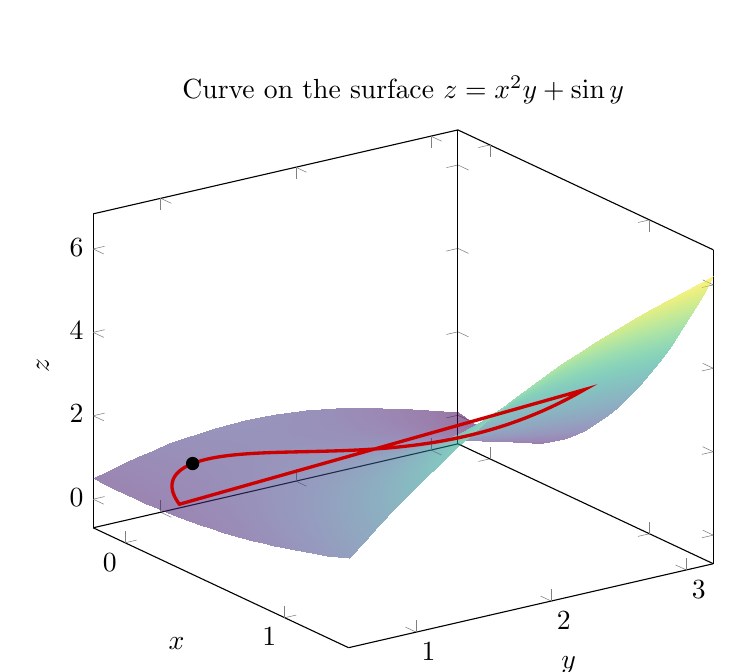
\begin{tikzpicture}
\begin{axis}[
  width=0.78\textwidth,
  view={55}{25},
  xlabel={$x$},ylabel={$y$},zlabel={$z$},
  domain=-0.2:1.4, y domain=0.5:3.2,
  samples=25,samples y=25,
  colormap/viridis,
  title={Curve on the surface $z=x^2y+\sin y$}
]
\addplot3[surf,opacity=0.55,shader=interp] {x^2*y + sin(deg(y))};
\addplot3[very thick,red!80!black,domain=-0.5:1.0,samples=120] ({x^2},{exp(x)},{(x^2)^2*exp(x)+sin(deg(exp(x)))});
\addplot3[only marks,mark=*,mark size=2.2pt] coordinates {(0,1,0.84147)};
\end{axis}
\end{tikzpicture}
\caption{The chain rule measures the rate at which a surface changes along a parameterized curve in the domain.}
\end{figure}

\section{The tree form of the chain rule}

Now suppose
\[
z=f(x,y),\qquad x=x(s,t),\qquad y=y(s,t).
\]
Then $z$ is a function of two variables $s$ and $t$:
\[
z(s,t)=f(x(s,t),y(s,t)).
\]
The partial derivatives of $z$ are
\[
\frac{\partial z}{\partial s}=\frac{\partial f}{\partial x}\frac{\partial x}{\partial s}+\frac{\partial f}{\partial y}\frac{\partial y}{\partial s},
\]
and
\[
\frac{\partial z}{\partial t}=\frac{\partial f}{\partial x}\frac{\partial x}{\partial t}+\frac{\partial f}{\partial y}\frac{\partial y}{\partial t}.
\]
A useful memory device is
\[
(s,t)\longrightarrow (x,y)\longrightarrow z.
\]
To differentiate $z$ with respect to one input variable, follow every path from that variable to $z$, multiply derivatives along each path, and add the path contributions.

\begin{figure}[H]
\centering
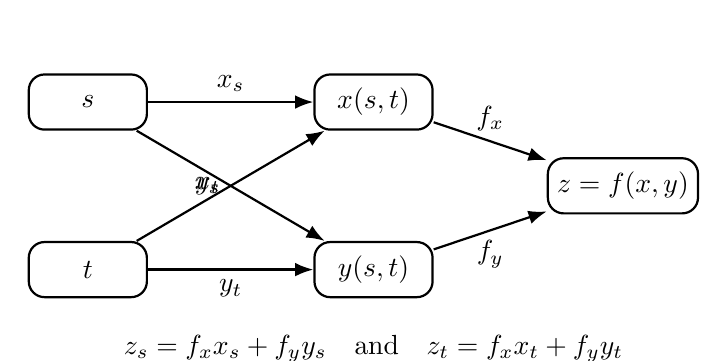
\begin{tikzpicture}[
  box/.style={draw,rounded corners=2mm,fill=white,minimum width=1.5cm,minimum height=0.7cm,align=center,thick},
  arrow/.style={-Latex,thick},
  node distance=1.4cm and 2.1cm
]
\node[box] (s) {$s$};
\node[box,below=of s] (t) {$t$};
\node[box,right=of s] (x) {$x(s,t)$};
\node[box,right=of t] (y) {$y(s,t)$};
\node[box,right=2.2cm of $(x)!0.5!(y)$] (z) {$z=f(x,y)$};
\draw[arrow] (s) -- node[above] {$x_s$} (x);
\draw[arrow] (s) -- node[left] {$y_s$} (y);
\draw[arrow] (t) -- node[left] {$x_t$} (x);
\draw[arrow] (t) -- node[below] {$y_t$} (y);
\draw[arrow] (x) -- node[above] {$f_x$} (z);
\draw[arrow] (y) -- node[below] {$f_y$} (z);
\node[below=0.35cm of y,align=center] {$z_s=f_xx_s+f_yy_s$\quad and\quad $z_t=f_xx_t+f_yy_t$};
\end{tikzpicture}
\caption{The tree form of the chain rule adds the derivative contribution from every dependency path.}
\end{figure}

\begin{workedexample}[Two-parameter chain rule]
Let
\[
f(x,y)=x^2+y^3,\qquad x=s+t,\qquad y=st.
\]
Then $f_x=2x$ and $f_y=3y^2$. Also
\[
x_s=1,\quad x_t=1,\quad y_s=t,\quad y_t=s.
\]
Therefore
\[
z_s=2x\cdot 1+3y^2\cdot t=2x+3ty^2,
\]
and
\[
z_t=2x\cdot 1+3y^2\cdot s=2x+3sy^2.
\]
Substituting $x=s+t$ and $y=st$ gives
\[
z_s=2(s+t)+3t(s^2t^2),\qquad z_t=2(s+t)+3s(s^2t^2).
\]
\end{workedexample}

\section{Jacobian matrices}

Let
\[
F:\R^n\to\R^m,
\]
where
\[
F(x_1,\dots,x_n)=\bmat{F_1(x_1,\dots,x_n)\\ \vdots\\ F_m(x_1,\dots,x_n)}.
\]
The \emph{Jacobian matrix} of $F$ is
\[
J_F(x)=
\begin{bmatrix}
\frac{\partial F_1}{\partial x_1} & \frac{\partial F_1}{\partial x_2} & \cdots & \frac{\partial F_1}{\partial x_n}\\
\frac{\partial F_2}{\partial x_1} & \frac{\partial F_2}{\partial x_2} & \cdots & \frac{\partial F_2}{\partial x_n}\\
\vdots & \vdots & \ddots & \vdots\\
\frac{\partial F_m}{\partial x_1} & \frac{\partial F_m}{\partial x_2} & \cdots & \frac{\partial F_m}{\partial x_n}
\end{bmatrix}.
\]
The entry in row $i$, column $j$ tells how the $i$th output changes when the $j$th input changes.

\begin{notebox}[Dimensions matter]
If $F:\R^n\to\R^m$, then $J_F$ is an $m\times n$ matrix. It maps small input displacements $\Delta x\in\R^n$ to small output displacements $\Delta F\in\R^m$:
\[
\Delta F\approx J_F(x)\Delta x.
\]
\end{notebox}

\begin{workedexample}[A Jacobian matrix]
Let
\[
F(x,y)=\bmat{x^2y\\ e^{x+y}\\ \sin(xy)}.
\]
Then $F:\R^2\to\R^3$. Its Jacobian is a $3\times 2$ matrix:
\[
J_F(x,y)=
\begin{bmatrix}
2xy & x^2\\
e^{x+y} & e^{x+y}\\
y\cos(xy) & x\cos(xy)
\end{bmatrix}.
\]
At $(1,0)$,
\[
J_F(1,0)=\begin{bmatrix}0&1\\ e&e\\ 0&1\end{bmatrix}.
\]
Thus if $(x,y)$ moves by a small vector $\Delta x=\langle h,k\rangle$, then
\[
\Delta F\approx
\begin{bmatrix}0&1\\ e&e\\ 0&1\end{bmatrix}
\begin{bmatrix}h\\k\end{bmatrix}
=\begin{bmatrix}k\\ e(h+k)\\ k\end{bmatrix}.
\]
\end{workedexample}

\section{The Jacobian as a local linear map}

For a scalar function $f:\R^n\to\R$, the derivative at a point is encoded by the gradient. For a vector-valued function $F:\R^n\to\R^m$, the derivative is encoded by the Jacobian. Near a point $a$,
\[
F(a+h)\approx F(a)+J_F(a)h.
\]
This means that the nonlinear function behaves like an affine linear map near $a$.

\begin{workedexample}[Local effect of a nonlinear map]
Let
\[
F(x,y)=\bmat{x+y\\ x^2-y}.
\]
Then
\[
J_F(x,y)=\begin{bmatrix}1&1\\2x&-1\end{bmatrix}.
\]
At $a=(1,1)$,
\[
J_F(1,1)=\begin{bmatrix}1&1\\2&-1\end{bmatrix}.
\]
Therefore a small square around $(1,1)$ in the input plane is approximately mapped to a parallelogram in the output plane.
\end{workedexample}

\begin{figure}[H]
\centering
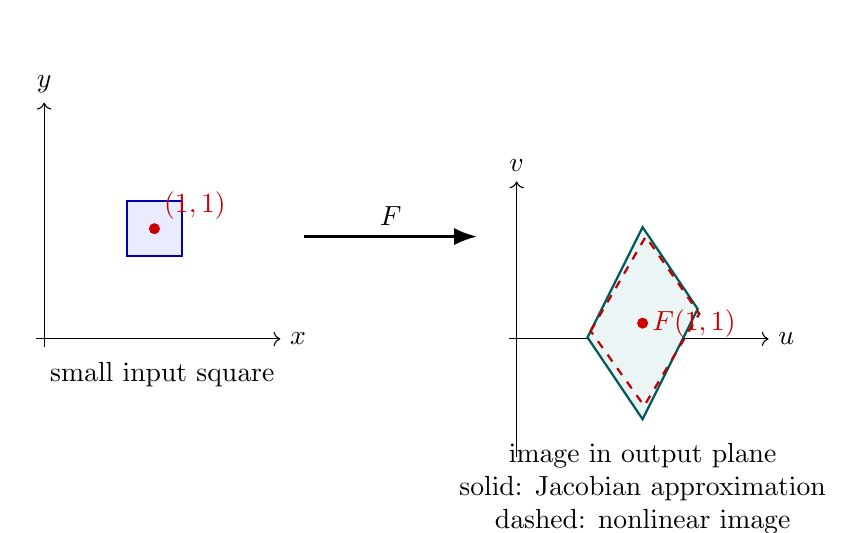
\begin{tikzpicture}[scale=1]
\begin{scope}
  \draw[->] (-0.1,0) -- (3.0,0) node[right] {$x$};
  \draw[->] (0,-0.1) -- (0,3.0) node[above] {$y$};
  \coordinate (a) at (1.4,1.4);
  \draw[thick,blue!70!black,fill=blue!8] ($(a)+(-0.35,-0.35)$)--($(a)+(0.35,-0.35)$)--($(a)+(0.35,0.35)$)--($(a)+(-0.35,0.35)$)--cycle;
  \fill[red!80!black] (a) circle (2pt) node[above right] {$(1,1)$};
  \node at (1.5,-0.45) {small input square};
\end{scope}
\begin{scope}[xshift=6.0cm]
  \draw[->] (-0.1,0) -- (3.2,0) node[right] {$u$};
  \draw[->] (0,-1.5) -- (0,2.0) node[above] {$v$};
  \coordinate (F) at (1.6,0.2);
  \coordinate (p1) at ($(F)+(-0.70,-0.18)$);
  \coordinate (p2) at ($(F)+(0.00,1.22)$);
  \coordinate (p3) at ($(F)+(0.70,0.18)$);
  \coordinate (p4) at ($(F)+(0.00,-1.22)$);
  \draw[thick,teal!70!black,fill=teal!8] (p1)--(p2)--(p3)--(p4)--cycle;
  \draw[thick,red!75!black,dashed] ($(F)+(-0.66,-0.10)$)--($(F)+(0.04,1.10)$)--($(F)+(0.72,0.12)$)--($(F)+(0.02,-1.05)$)--cycle;
  \fill[red!80!black] (F) circle (2pt) node[right] {$F(1,1)$};
  \node[align=center] at (1.6,-1.9) {image in output plane\\solid: Jacobian approximation\\dashed: nonlinear image};
\end{scope}
\draw[-Latex,very thick] (3.3,1.3) -- node[above] {$F$} (5.5,1.3);
\end{tikzpicture}
\caption{Near a point, a nonlinear map is approximated by its Jacobian linear map.}
\end{figure}

\section{Matrix form of the chain rule}

Suppose
\[
F:\R^n\to\R^m,\qquad G:\R^m\to\R^p.
\]
Then the composition $G\circ F:\R^n\to\R^p$ has Jacobian
\begin{formulabox}[Matrix chain rule]
\[
\boxed{J_{G\circ F}(x)=J_G(F(x))J_F(x)}.
\]
The order is important: first apply $F$, then apply $G$, but the Jacobian matrices multiply as outer derivative times inner derivative.
\end{formulabox}
This is the multivariable version of $(g\circ f)'(x)=g'(f(x))f'(x)$.

\begin{workedexample}[Matrix chain rule]
Let
\[
F(s,t)=\bmat{x\\y}=\bmat{s+t\\ st},
\qquad
G(x,y)=x^2+y^3.
\]
The Jacobian of $F$ is
\[
J_F(s,t)=\begin{bmatrix}1&1\\t&s\end{bmatrix}.
\]
The Jacobian of $G$ is the row vector
\[
J_G(x,y)=\begin{bmatrix}2x&3y^2\end{bmatrix}.
\]
Therefore
\[
J_{G\circ F}(s,t)=\begin{bmatrix}2x&3y^2\end{bmatrix}
\begin{bmatrix}1&1\\t&s\end{bmatrix}
=\begin{bmatrix}2x+3ty^2&2x+3sy^2\end{bmatrix}.
\]
This matches the tree form of the chain rule.
\end{workedexample}

\section{Gradients through linear maps}

A very common situation in data science and machine learning is
\[
L(w)=\phi(Aw+b),
\]
where $w\in\R^n$ is a parameter vector, $A$ is a matrix, $b$ is a vector, and $\phi$ is a scalar loss function. Let
\[
u=Aw+b.
\]
Then the chain rule gives
\begin{formulabox}[Gradient through a linear map]
\[
\boxed{\grad_w L(w)=A^T\grad_u\phi(u)},\qquad u=Aw+b.
\]
The value moves forward through $u=Aw+b$. The gradient moves backward through $A^T$.
\end{formulabox}

\begin{workedexample}[Least-squares gradient]
Let
\[
L(w)=\frac12\|Xw-y\|^2,
\]
where $X$ is a data matrix, $w$ is a parameter vector, and $y$ is an observed response vector. Define $r=Xw-y$. Then
\[
L=\frac12 r^Tr.
\]
The gradient with respect to $r$ is $\grad_r L=r$. Since $r=Xw-y$, the chain rule gives
\[
\boxed{\grad_w L=X^T(Xw-y)}.
\]
This is one of the most important gradients in applied mathematics, statistics, and machine learning.
\end{workedexample}

\begin{figure}[H]
\centering
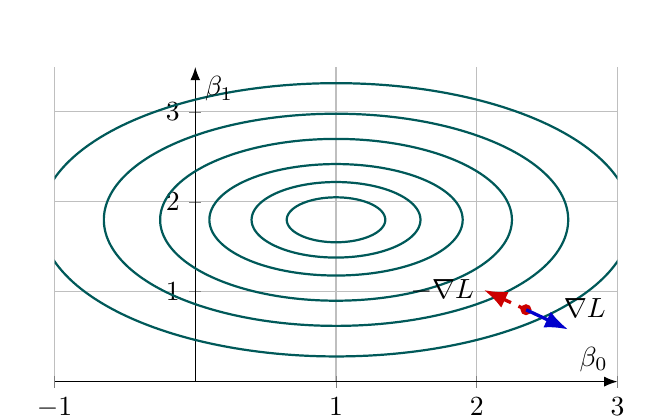
\begin{tikzpicture}
\begin{axis}[
  width=0.72\textwidth,
  height=0.46\textwidth,
  xmin=-1,xmax=3,
  ymin=0,ymax=3.5,
  axis lines=middle,
  xlabel={$\beta_0$},ylabel={$\beta_1$},
  grid=both,
  axis line style={-Latex}
]
\foreach \a/\b in {0.35/0.25,0.6/0.42,0.9/0.62,1.25/0.9,1.65/1.18,2.1/1.52}{
  \addplot[domain=0:360,samples=220,teal!70!black,thick] ({1.0 + \a*cos(x)},{1.8 + \b*sin(x)});
}
\fill[red!80!black] (axis cs:2.35,0.8) circle (2pt);
\addplot[blue!80!black,very thick,-Latex] coordinates {(2.35,0.8) (2.65,0.58)};
\addplot[red!80!black,very thick,dashed,-Latex] coordinates {(2.35,0.8) (2.05,1.02)};
\node[above right] at (axis cs:2.55,0.6) {$\grad L$};
\node[left] at (axis cs:2.05,1.02) {$-\grad L$};
\end{axis}
\end{tikzpicture}
\caption{The least-squares gradient points toward increasing loss, while gradient descent moves in the opposite direction.}
\end{figure}

\section{Numerical Jacobians by finite differences}

In applications, we may have a function implemented as code but not have a closed formula. We can approximate the Jacobian using finite differences. For $F:\R^n\to\R^m$, the $j$th column of the Jacobian can be approximated by
\[
\frac{F(x+he_j)-F(x-he_j)}{2h},
\]
where $e_j$ is the $j$th standard basis vector.

\begin{figure}[H]
\centering
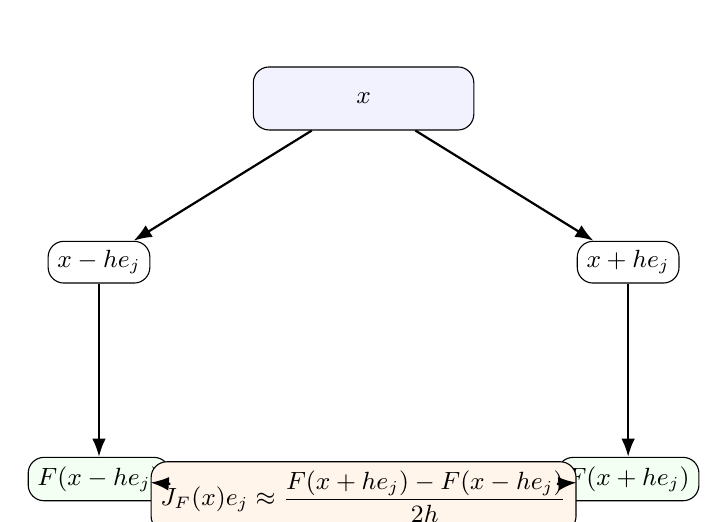
\begin{tikzpicture}[font=\small]
\node[draw,rounded corners=2mm,fill=blue!5,minimum width=2.8cm,minimum height=0.8cm] (x) {$x$};
\node[draw,rounded corners=2mm,fill=white,below left=1.4cm and 1.3cm of x] (xm) {$x-he_j$};
\node[draw,rounded corners=2mm,fill=white,below right=1.4cm and 1.3cm of x] (xp) {$x+he_j$};
\node[draw,rounded corners=2mm,fill=green!5,below=2.2cm of xm] (fm) {$F(x-he_j)$};
\node[draw,rounded corners=2mm,fill=green!5,below=2.2cm of xp] (fp) {$F(x+he_j)$};
\node[draw,rounded corners=2mm,fill=orange!8,below=4.2cm of x,minimum width=5.2cm] (col) {$\displaystyle J_F(x)e_j\approx \frac{F(x+he_j)-F(x-he_j)}{2h}$};
\draw[-Latex,thick] (x) -- (xm);
\draw[-Latex,thick] (x) -- (xp);
\draw[-Latex,thick] (xm) -- (fm);
\draw[-Latex,thick] (xp) -- (fp);
\draw[-Latex,thick] (fm) -- (col);
\draw[-Latex,thick] (fp) -- (col);
\end{tikzpicture}
\caption{A centered finite difference estimates one column of the Jacobian at a time.}
\end{figure}

Finite differences are useful, but they can be slow or unstable for very large models. Automatic differentiation gives a more efficient and accurate way to compute derivatives of functions defined by code.

\section{Computational graphs}

A \emph{computational graph} breaks a complicated function into elementary operations. Each node stores a value. Each edge represents dependence.

Consider
\[
f(x,y)=(xy+\sin x)^2.
\]
We can compute it step by step:
\[
a=xy,\qquad b=\sin x,\qquad c=a+b,\qquad f=c^2.
\]
The chain rule can be applied locally at every step.

\begin{workedexample}[Forward sensitivity]
For $f(x,y)=(xy+\sin x)^2$, set
\[
a=xy,\qquad b=\sin x,\qquad c=a+b,\qquad f=c^2.
\]
Then
\[
\frac{\partial f}{\partial c}=2c,
\qquad
\frac{\partial c}{\partial a}=1,
\qquad
\frac{\partial c}{\partial b}=1,
\]
and
\[
\frac{\partial a}{\partial x}=y,
\qquad
\frac{\partial a}{\partial y}=x,
\qquad
\frac{\partial b}{\partial x}=\cos x.
\]
Therefore
\[
\frac{\partial f}{\partial x}=2c(y+\cos x),
\qquad
\frac{\partial f}{\partial y}=2cx.
\]
Since $c=xy+\sin x$,
\[
\grad f(x,y)=\left\langle 2(xy+\sin x)(y+\cos x),\;2x(xy+\sin x)\right\rangle.
\]
\end{workedexample}

\begin{figure}[H]
\centering
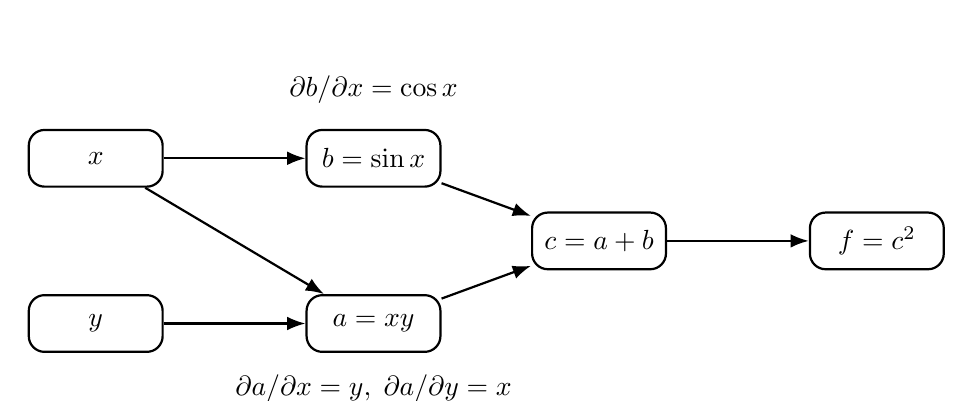
\begin{tikzpicture}[
  box/.style={draw,rounded corners=2mm,fill=white,minimum width=1.7cm,minimum height=0.72cm,align=center,thick},
  arrow/.style={-Latex,thick},
  node distance=1.35cm and 1.8cm
]
\node[box] (x) {$x$};
\node[box,below=of x] (y) {$y$};
\node[box,right=of y] (a) {$a=xy$};
\node[box,right=of x] (b) {$b=\sin x$};
\node[box,right=2.0cm of $(a)!0.5!(b)$] (c) {$c=a+b$};
\node[box,right=of c] (f) {$f=c^2$};
\draw[arrow] (x) -- (a);
\draw[arrow] (y) -- (a);
\draw[arrow] (x) -- (b);
\draw[arrow] (a) -- (c);
\draw[arrow] (b) -- (c);
\draw[arrow] (c) -- (f);
\node[above=0.2cm of b] {$\partial b/\partial x=\cos x$};
\node[below=0.15cm of a] {$\partial a/\partial x=y,\;\partial a/\partial y=x$};
\end{tikzpicture}
\caption{A computational graph decomposes a function into elementary operations where local derivatives are easy to compute.}
\end{figure}

\section{Reverse-mode automatic differentiation}

Automatic differentiation is not symbolic differentiation and not finite differences. It computes exact derivatives of the operations performed by a program, up to floating-point rounding.

There are two main modes:
\begin{itemize}
  \item \emph{Forward mode} propagates derivatives from inputs to outputs.
  \item \emph{Reverse mode} propagates derivatives from output back to inputs.
\end{itemize}
Reverse mode is especially efficient when there is one scalar output and many inputs, which is exactly the situation for many loss functions:
\[
L(\theta_1,\dots,\theta_n):\R^n\to\R.
\]
Backpropagation is reverse-mode automatic differentiation applied to neural networks.

\begin{workedexample}[Reverse accumulation]
Again let
\[
f=(xy+\sin x)^2.
\]
At each node, reverse mode stores an \emph{adjoint}, meaning the derivative of the final output with respect to that node. Start with
\[
\bar f=\frac{\partial f}{\partial f}=1.
\]
Since $f=c^2$,
\[
\bar c=\bar f\frac{\partial f}{\partial c}=2c.
\]
Since $c=a+b$,
\[
\bar a=\bar c,\qquad \bar b=\bar c.
\]
Since $a=xy$ and $b=\sin x$,
\[
\bar x=\bar a\,y+\bar b\,\cos x,
\qquad
\bar y=\bar a\,x.
\]
This gives the same gradient as before, but the organization is different: compute values forward, then gradients backward.
\end{workedexample}

\begin{figure}[H]
\centering
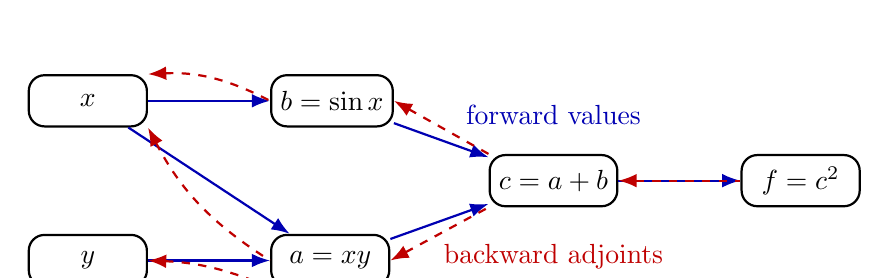
\begin{tikzpicture}[
  box/.style={draw,rounded corners=2mm,fill=white,minimum width=1.5cm,minimum height=0.65cm,align=center,thick},
  fwd/.style={-Latex,thick,blue!70!black},
  rev/.style={Latex-,thick,red!75!black,dashed},
  node distance=1.35cm and 1.55cm
]
\node[box] (x) {$x$};
\node[box,below=of x] (y) {$y$};
\node[box,right=of y] (a) {$a=xy$};
\node[box,right=of x] (b) {$b=\sin x$};
\node[box,right=2.0cm of $(a)!0.5!(b)$] (c) {$c=a+b$};
\node[box,right=of c] (f) {$f=c^2$};
\draw[fwd] (x) -- (a); \draw[fwd] (y) -- (a); \draw[fwd] (x) -- (b); \draw[fwd] (a) -- (c); \draw[fwd] (b) -- (c); \draw[fwd] (c) -- (f);
\draw[rev] (x.south east) to[bend right=15] (a.west);
\draw[rev] (y.east) to[bend left=10] (a.south west);
\draw[rev] (x.north east) to[bend left=15] (b.west);
\draw[rev] (a.east) -- (c.south west);
\draw[rev] (b.east) -- (c.north west);
\draw[rev] (c.east) -- (f.west);
\node[blue!70!black,above=0.25cm of c] {forward values};
\node[red!75!black,below=0.35cm of c] {backward adjoints};
\end{tikzpicture}
\caption{Reverse mode first evaluates the graph forward, then propagates adjoints backward from the scalar output.}
\end{figure}

\section{A tiny neural-network example}

Consider a very small model with one input $x$, one weight $w$, one bias $b$, and sigmoid activation
\[
\widehat y=\sigma(wx+b),
\qquad
\sigma(u)=\frac{1}{1+e^{-u}}.
\]
For a target value $y$, use the squared loss
\[
L(w,b)=\frac12(\widehat y-y)^2.
\]
The computation is
\[
u=wx+b,\qquad \widehat y=\sigma(u),\qquad L=\frac12(\widehat y-y)^2.
\]
The chain rule gives
\[
\frac{\partial L}{\partial w}=(\widehat y-y)\sigma'(u)x,
\qquad
\frac{\partial L}{\partial b}=(\widehat y-y)\sigma'(u),
\]
where
\[
\sigma'(u)=\sigma(u)(1-\sigma(u)).
\]
This is backpropagation in its smallest possible form.

\begin{figure}[H]
\centering
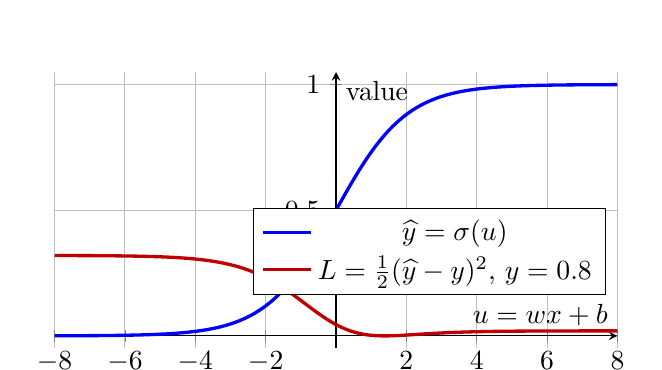
\begin{tikzpicture}
\begin{axis}[
  width=0.72\textwidth,
  height=0.42\textwidth,
  xmin=-8,xmax=8,
  ymin=-0.05,ymax=1.05,
  axis lines=middle,
  xlabel={$u=wx+b$},
  ylabel={value},
  grid=both,
  legend style={at={(0.98,0.35)},anchor=east,fill=white}
]
\addplot[very thick,blue,domain=-8:8,samples=300] {1/(1+exp(-x))};
\addlegendentry{$\widehat y=\sigma(u)$}
\addplot[very thick,red!75!black,domain=-8:8,samples=300] {0.5*(1/(1+exp(-x))-0.8)^2};
\addlegendentry{$L=\frac12(\widehat y-y)^2$, $y=0.8$}
\end{axis}
\end{tikzpicture}
\caption{A one-neuron model is a composition of an affine map, a nonlinear activation, and a loss function.}
\end{figure}

\section{Chain rule and coordinate transformations}

Coordinate transformations are also compositions. For polar coordinates,
\[
x=r\cos\theta,\qquad y=r\sin\theta.
\]
If $z=f(x,y)$, then
\[
z(r,\theta)=f(r\cos\theta,r\sin\theta).
\]
The chain rule gives
\[
\frac{\partial z}{\partial r}=f_x\cos\theta+f_y\sin\theta,
\]
and
\[
\frac{\partial z}{\partial \theta}=f_x(-r\sin\theta)+f_y(r\cos\theta).
\]
The Jacobian matrix of the polar coordinate map
\[
\Phi(r,\theta)=\bmat{r\cos\theta\\r\sin\theta}
\]
is
\[
J_\Phi(r,\theta)=\begin{bmatrix}\cos\theta&-r\sin\theta\\ \sin\theta&r\cos\theta\end{bmatrix}.
\]
Its determinant is
\[
\det J_\Phi(r,\theta)=r.
\]
This determinant explains why the area element becomes
\[
dA=r\,dr\,d\theta.
\]
Thus the chain rule for derivatives and the change-of-variables rule for integrals are closely connected.

\begin{figure}[H]
\centering
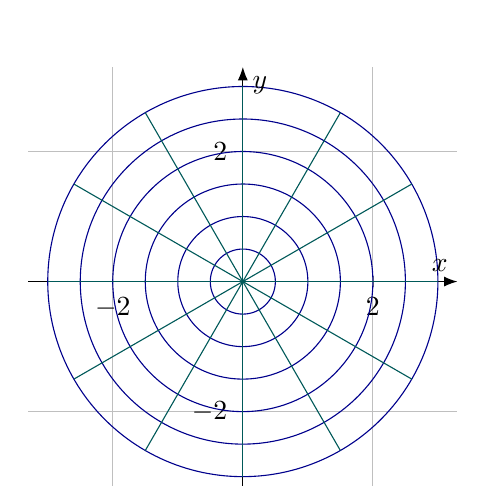
\begin{tikzpicture}
\begin{axis}[
  width=0.58\textwidth,
  height=0.58\textwidth,
  xmin=-3.3,xmax=3.3,
  ymin=-3.3,ymax=3.3,
  axis equal image,
  axis lines=middle,
  xlabel={$x$},ylabel={$y$},
  grid=both,
  axis line style={-Latex}
]
\foreach \r in {0.5,1.0,1.5,2.0,2.5,3.0}{
  \addplot[domain=0:360,samples=220,blue!55!black] ({\r*cos(x)},{\r*sin(x)});
}
\foreach \ang in {0,30,...,330}{
  \addplot[domain=0:3,samples=50,teal!70!black] ({x*cos(\ang)},{x*sin(\ang)});
}
\end{axis}
\end{tikzpicture}
\caption{The polar coordinate map bends a rectangular grid in parameter space into radial and circular coordinate curves.}
\end{figure}

\section{Implicit differentiation as a chain rule}

Suppose $z=z(x,y)$ is defined implicitly by
\[
F(x,y,z)=0.
\]
Then $F(x,y,z(x,y))$ is identically zero. Differentiating with respect to $x$ gives
\[
F_x+F_z\frac{\partial z}{\partial x}=0.
\]
Therefore, if $F_z\ne 0$,
\[
\boxed{\frac{\partial z}{\partial x}=-\frac{F_x}{F_z}}.
\]
Similarly,
\[
\boxed{\frac{\partial z}{\partial y}=-\frac{F_y}{F_z}}.
\]
This is the same chain rule idea, but now one variable is hidden inside an equation.

\begin{workedexample}[Implicit partial derivatives]
Suppose $z=f(x,y)$ is defined by
\[
x^3+y^3+z^3+2xyz=3.
\]
Let
\[
F(x,y,z)=x^3+y^3+z^3+2xyz-3.
\]
Then
\[
F_x=3x^2+2yz,
\qquad
F_y=3y^2+2xz,
\qquad
F_z=3z^2+2xy.
\]
Thus
\[
\frac{\partial z}{\partial x}=-\frac{3x^2+2yz}{3z^2+2xy},
\qquad
\frac{\partial z}{\partial y}=-\frac{3y^2+2xz}{3z^2+2xy}.
\]
\end{workedexample}

\section{Common mistakes}

\begin{warningbox}[Mistake 1: Forgetting all paths]
If $z=f(x,y)$ and both $x$ and $y$ depend on $t$, then $dz/dt$ has two contributions:
\[
\frac{dz}{dt}=f_xx'(t)+f_yy'(t).
\]
Do not keep only one path.
\end{warningbox}

\begin{warningbox}[Mistake 2: Multiplying Jacobians in the wrong order]
For $G\circ F$, the derivative is
\[
J_{G\circ F}(x)=J_G(F(x))J_F(x),
\]
not $J_F(x)J_G(F(x))$. Check matrix dimensions.
\end{warningbox}

\begin{warningbox}[Mistake 3: Confusing gradient and Jacobian]
For a scalar-valued function $f:\R^n\to\R$, the Jacobian is a $1\times n$ row vector, while the gradient is usually written as an $n\times 1$ column vector or as a vector in $\R^n$. The information is the same, but the orientation matters in matrix formulas.
\end{warningbox}

\begin{warningbox}[Mistake 4: Treating automatic differentiation as numerical differentiation]
Finite differences estimate derivatives by evaluating nearby points. Automatic differentiation applies the chain rule exactly to the operations in a program. These are different methods.
\end{warningbox}

\section{Summary of core formulas}

\begin{formulabox}[Chain rule along a curve]
If $z=f(x(t),y(t))$, then
\[
\frac{dz}{dt}=f_x\frac{dx}{dt}+f_y\frac{dy}{dt},
\qquad
\frac{d}{dt}f(r(t))=\grad f(r(t))\cdot r'(t).
\]
\end{formulabox}

\begin{formulabox}[Chain rule with two parameters]
If $z=f(x(s,t),y(s,t))$, then
\[
z_s=f_xx_s+f_yy_s,
\qquad
z_t=f_xx_t+f_yy_t.
\]
\end{formulabox}

\begin{formulabox}[Jacobian matrix and linear approximation]
For $F:\R^n\to\R^m$,
\[
J_F(x)=\left[\frac{\partial F_i}{\partial x_j}\right],
\qquad
F(a+h)\approx F(a)+J_F(a)h.
\]
\end{formulabox}

\begin{formulabox}[Matrix chain rule]
\[
J_{G\circ F}(x)=J_G(F(x))J_F(x).
\]
\end{formulabox}

\begin{formulabox}[Gradient through a linear map]
If $L(w)=\phi(Aw+b)$, then
\[
\grad_w L=A^T\grad_u\phi(u),\qquad u=Aw+b.
\]
\end{formulabox}

\begin{formulabox}[Implicit differentiation]
If $F(x,y,z(x,y))=0$, then
\[
z_x=-\frac{F_x}{F_z},
\qquad
z_y=-\frac{F_y}{F_z}.
\]
\end{formulabox}

\section{Practice problems}

\subsection*{Conceptual problems}
\begin{enumerate}
  \item Explain why the chain rule is a rule about composition.
  \item Explain why the chain rule adds contributions from different paths in a dependency graph.
  \item What is the dimension of the Jacobian matrix for a map $F:\R^5\to\R^3$?
  \item Explain the difference between a gradient and a Jacobian.
  \item Why does reverse-mode automatic differentiation work well for scalar loss functions with many parameters?
  \item Explain why $A^T$ appears when backpropagating a gradient through $u=Aw+b$.
\end{enumerate}

\subsection*{Computational and algebraic problems}
\begin{enumerate}[start=7]
  \item Let $z=x^2+xy+y^2$, where $x=t^2$ and $y=\sin t$. Find $dz/dt$.
  \item Let $z=e^{xy}$, where $x=s+t$ and $y=s-t$. Find $z_s$ and $z_t$.
  \item Let $F(x,y)=\langle x^2+y,xy,\sin(x+y)\rangle$. Compute $J_F(x,y)$.
  \item Let $F(x,y)=\langle x+y,x-y\rangle$ and $G(u,v)=u^2+v^2$. Compute $J_{G\circ F}$ using matrix multiplication.
  \item Let $F(x,y,z)=x^2+y^2+z^2-1=0$ define $z=z(x,y)$ near a point with $z\ne 0$. Find $z_x$ and $z_y$.
  \item Let $L(w)=\frac12\|Aw-y\|^2$. Derive $\grad_w L=A^T(Aw-y)$.
  \item For $f(x,y)=(x^2+y)^3$, draw a computational graph and compute $\grad f$ by the chain rule.
  \item For $\widehat y=\sigma(w_1x_1+w_2x_2+b)$ and $L=\frac12(\widehat y-y)^2$, compute $\partial L/\partial w_1$, $\partial L/\partial w_2$, and $\partial L/\partial b$.
  \item Use finite differences to approximate the Jacobian of $F(x,y)=\langle e^{xy},x^2-y^2\rangle$ at $(1,2)$.
\end{enumerate}

\subsection*{Challenge problems}
\begin{enumerate}[start=16]
  \item Let $F:\R^2\to\R^2$ be $F(r,\theta)=\langle r\cos\theta,r\sin\theta\rangle$. Compute $J_F$ and explain geometrically why $|\det J_F|=r$.
  \item Let $F(x)=Ax$ and $G(u)=\frac12\|u-y\|^2$. Use the matrix chain rule to derive the least-squares gradient.
  \item Suppose $H=G\circ F$ where $F:\R^n\to\R^m$ and $G:\R^m\to\R$. Show that $\grad H(x)=J_F(x)^T\grad G(F(x))$ when gradients are written as column vectors.
  \item Write a short paragraph explaining how backpropagation is related to the chain rule.
  \item Consider $f(x,y,z)=\sin(xy)+z^2$ and a curve $r(t)=\langle t,e^t,\cos t\rangle$. Compute $d(f\circ r)/dt$ at $t=0$.
\end{enumerate}

\section{Python lab and interactive page}

\begin{itemize}
  \item Notebook lab: \texttt{\small Chapter10\_Chain\_Rule\_Jacobians\_and\_Automatic\_Differentiation.ipynb}
  \item Interactive HTML page: \texttt{../htmls/chapter-10.html}
\end{itemize}

\section{Chapter summary}

The chain rule is the calculus of composition. In its simplest form, it differentiates $f(g(t))$. In multivariable calculus, it differentiates functions passing through curves, surfaces, coordinate transformations, and computational graphs. The Jacobian matrix organizes these derivative calculations as linear maps. The matrix chain rule
\[
J_{G\circ F}(x)=J_G(F(x))J_F(x)
\]
is the central formula of the chapter.

For modern applied mathematics, statistics, and machine learning, the most important lesson is that derivatives can be propagated through models. Least-squares gradients, logistic-regression gradients, neural-network backpropagation, coordinate transformations, and sensitivity analysis are all expressions of the same idea: compute local derivatives at each step and combine them by the chain rule.

\end{document}
